\documentclass[compress]{beamer}
\usetheme{sthlm}

%-=-=-=-=-=-=-=-=-=-=-=-=-=-=-=-=-=-=-=-=-=-=-=-=
%        LOADING BEAMER PACKAGES
%-=-=-=-=-=-=-=-=-=-=-=-=-=-=-=-=-=-=-=-=-=-=-=-=

\usepackage{
booktabs,
datetime,
dtk-logos,
graphicx,
multicol,
pgfplots,
ragged2e,
tabularx,
tikz,
wasysym,
multirow,
float,
caption,
subcaption
}

\pgfplotsset{compat=1.8}

\usepackage[utf8]{inputenc}
\usepackage[portuguese]{babel}
\usepackage[T1]{fontenc}
\usepackage{newpxtext,newpxmath}
\usepackage{listings}

\lstset{ %
language=[LaTeX]TeX,
basicstyle=\normalsize\ttfamily,
keywordstyle=,
numbers=left,
numberstyle=\tiny\ttfamily,
stepnumber=1,
showspaces=false,
showstringspaces=false,
showtabs=false,
breaklines=true,
frame=tb,
framerule=0.5pt,
tabsize=4,
framexleftmargin=0.5em,
framexrightmargin=0.5em,
xleftmargin=0.5em,
xrightmargin=0.5em
}



%-=-=-=-=-=-=-=-=-=-=-=-=-=-=-=-=-=-=-=-=-=-=-=-=
%        LOADING TIKZ LIBRARIES
%-=-=-=-=-=-=-=-=-=-=-=-=-=-=-=-=-=-=-=-=-=-=-=-=

\usetikzlibrary{
backgrounds,
mindmap
}

%-=-=-=-=-=-=-=-=-=-=-=-=-=-=-=-=-=-=-=-=-=-=-=-=
%        BEAMER OPTIONS
%-=-=-=-=-=-=-=-=-=-=-=-=-=-=-=-=-=-=-=-=-=-=-=-=

\setbeameroption{show notes}

%-=-=-=-=-=-=-=-=-=-=-=-=-=-=-=-=-=-=-=-=-=-=-=-=
%        BEAMER COMMANDS
%-=-=-=-=-=-=-=-=-=-=-=-=-=-=-=-=-=-=-=-=-=-=-=-=


%-=-=-=-=-=-=-=-=-=-=-=-=-=-=-=-=-=-=-=-=-=-=-=-=
%
%	PRESENTATION INFORMATION
%
%-=-=-=-=-=-=-=-=-=-=-=-=-=-=-=-=-=-=-=-=-=-=-=-=

\title{Remote Procedure Calls}
\subtitle{DCE540 - Computação Paralela e Distribuída}
%\date{\small{\jobname}}
\author{\texttt{Iago Carvalho}}
\institute{\texttt{Departamento de Ciência da Computação}}

\hypersetup{
pdfauthor = {Iago A. Carvalho},      
pdfsubject = {Computação Paralela e Distribuída},
pdfkeywords = {},  
pdfmoddate= {D:\pdfdate},          
pdfcreator = {WriteLaTeX}
}

\begin{document}

\begin{frame}
\titlepage

\end{frame}

%% --------------------------------------------------------

\begin{frame}{Remote Procedure Calls (RPC)}

Comunicação transiente + mensagens síncronas \textcolor{sthlmDarkBlue}{$\rightarrow$} RPC

\vspace{0.5cm}

De forma simplificada, uma RPC permite que um componente \textit{A} chame um método de outro componente \textit{B}
\begin{itemize}
    \item \textit{A} e \textit{B} localizados em diferentes nós do sistema
    \item Total transparência ao desenvolvedor
\end{itemize}

\vspace{0.25cm}

\centering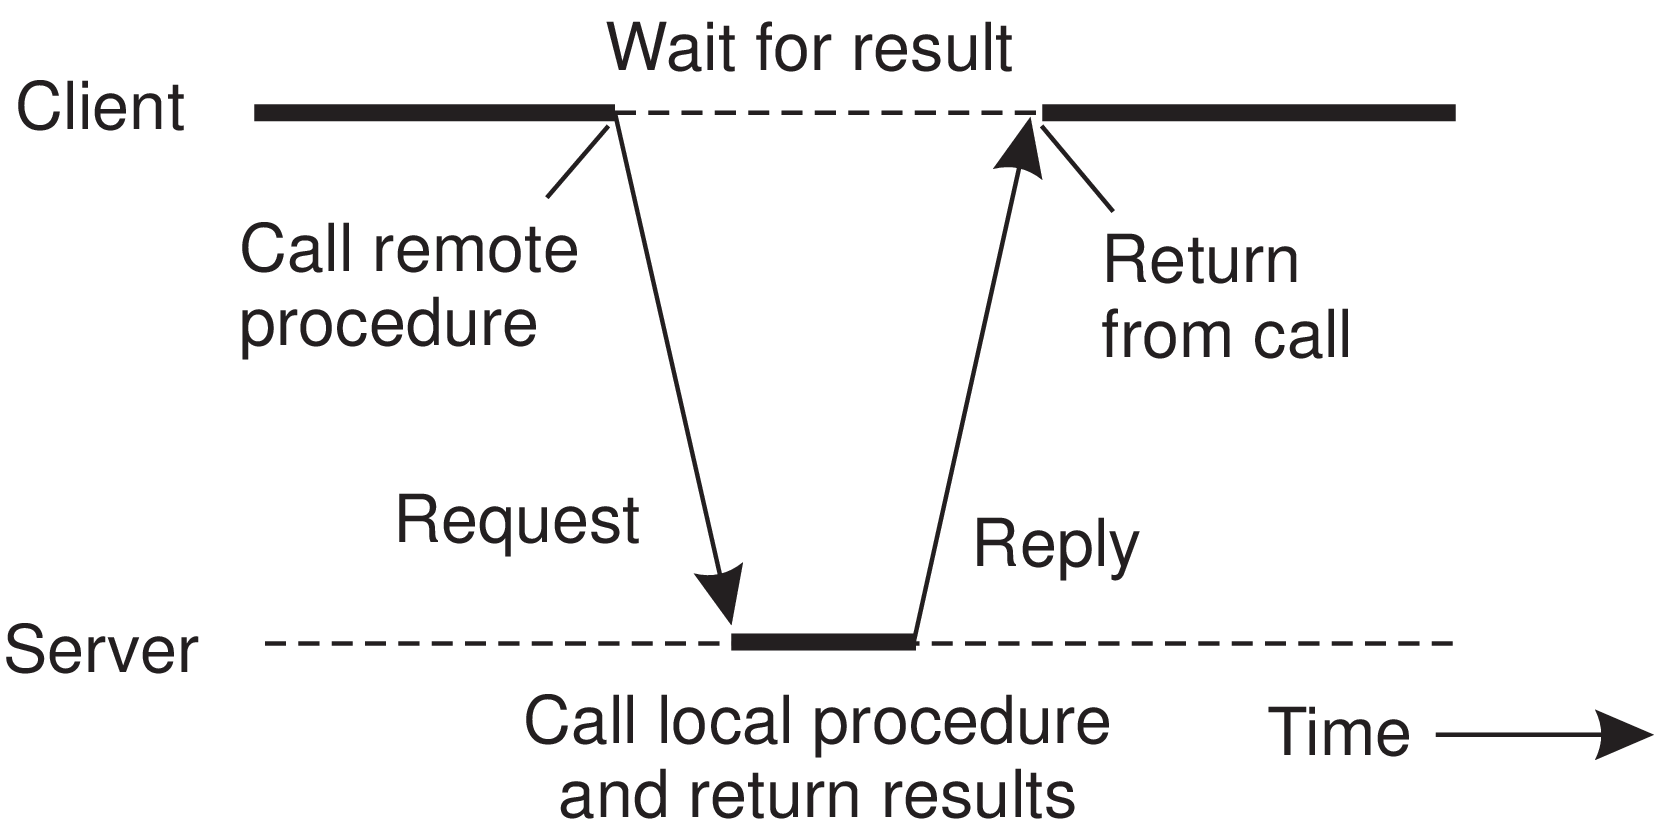
\includegraphics[width=0.8\textwidth]{images/rpc.png}

\end{frame}


%% --------------------------------------------------------

\begin{frame}{Remote Procedure Call - Problemas}

Inicialmente, a ideia parece simples e elegante (e de fato é) \\
Entretanto, existem alguns problemas crônicos com RPCs

\vspace{0.5cm}

\begin{itemize}
    \item Diferentes endereços (diferentes nós de rede)
    \item Passagem de parâmetros
    \item Possibilidade de uma das máquinas estar desligada
\end{itemize}


\end{frame}

%% --------------------------------------------------------

\begin{frame}[fragile]{Funcionamento básico}

É possível fazer um paralelo de uma RPC em um sistema distribuído para chamadas locais de um \textit{software} em um ambiente não-distribuído

Um \textit{software} quer 
\begin{enumerate}
    \item Ter acesso a uma lista
    \item Incluir um novo item 
    \item Obter uma referência para a nova lista
\end{enumerate}

\begin{verbatim}
novaLista = append(novoItem, listaAntiga)
\end{verbatim}

\end{frame}

%% --------------------------------------------------------

\begin{frame}{Funcionamento básico}

\vspace{0.5cm}

\centering 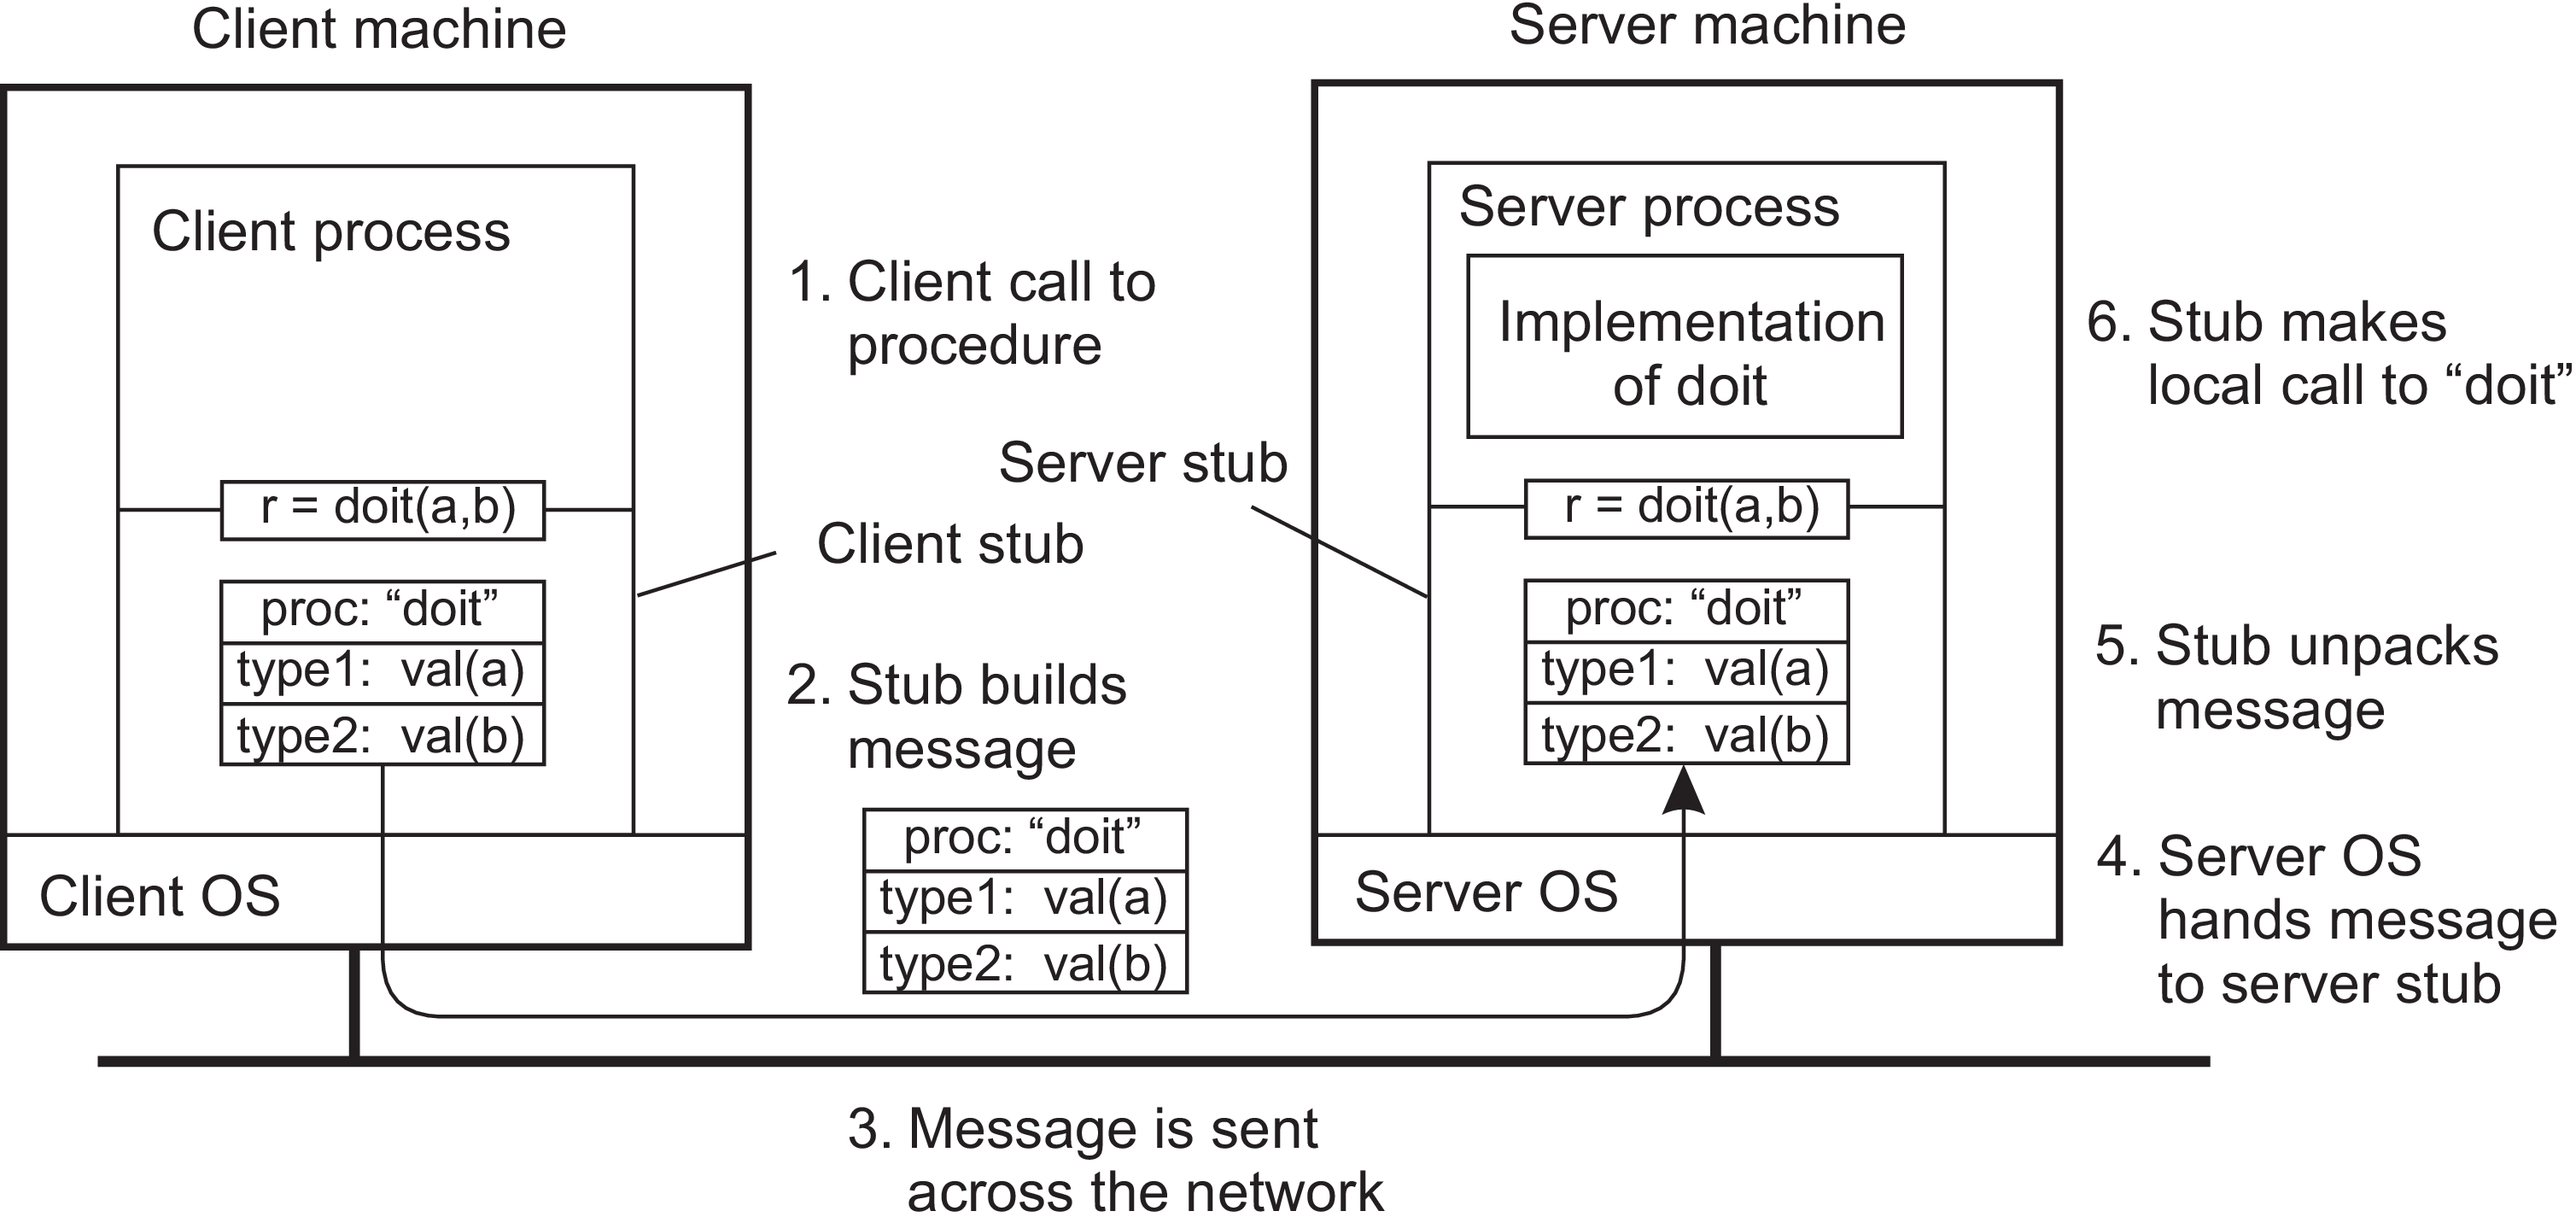
\includegraphics[width=\textwidth]{images/rpc_operation.png}

\end{frame}

%% --------------------------------------------------------

\begin{frame}[fragile]{Passagem de parâmetros}

É possível chamar um método utilizando uma RPC
\begin{itemize}
    \item Método aceita parâmetros
\end{itemize}

\vspace{0.5cm}

Em ambientes tradicionais, parâmetros são passados diretamente na chamada do método

\begin{verbatim}
    novaLista = append(novoItem, listaAntiga)
\end{verbatim}

Entretanto, em ambientes distribuídos, tudo o que é transferido é uma sequência  de bits
\begin{itemize}
    \item O servidor tem que ser capaz de entender e processar corretamente os parâmetros enviados
\end{itemize}
\end{frame}

%% --------------------------------------------------------

\begin{frame}[fragile]{Passagem de parâmetros}

O que é preciso para realizar a passagem de parâmetros?
\begin{itemize}
    \item Deve-se transformar os parâmetros em um formato padronizado
    \begin{itemize}
        \item Independente de arquitetura dos nós envolvidos
        \item Independente da rede
    \end{itemize}
    \item Ambos os componentes envolvidos tem que saber o tipo de parâmetro que está sendo enviado
\end{itemize}

\vspace{0.5cm}

Para isto, o \textit{middleware} que implementa uma RPC deve ser capaz de fornecer mecanismos de
\begin{itemize}
    \item Empacotar parâmetros
    \item Desempacotar parâmetros
\end{itemize}
\end{frame}

%% --------------------------------------------------------

\begin{frame}{Passagem de endereços de memória (ponteiros)}

É impossível realizar a passagem de ponteiros da maneira como conhecemos
\begin{itemize}
    \item Quando o servidor obter o parâmetro, ele indicará uma coisa completamente diferente
\end{itemize}

\vspace{0.5cm}

Solução: criar uma cópia do conteúdo que está na memória
\begin{itemize}
    \item Enviar esta cópia
\end{itemize}

Mas ainda existe outra solução...
\end{frame}

%% --------------------------------------------------------

\begin{frame}{Referências globais}

Caso exista um servidor de arquivos em comum, é possível criar referências globais
\begin{itemize}
    \item Espaço de endereçamento de memória comum a todos os componentes
\end{itemize}

Isto é possível quando os diversos componentes acessam dados de um mesmo local
\begin{itemize}
    \item Componente de dados
    \item Nó responsável por armazenar dados
    \item $\ldots$
\end{itemize}
\end{frame}

%% --------------------------------------------------------

\begin{frame}{RPC assíncrona}

\vspace{0.5cm}

\centering 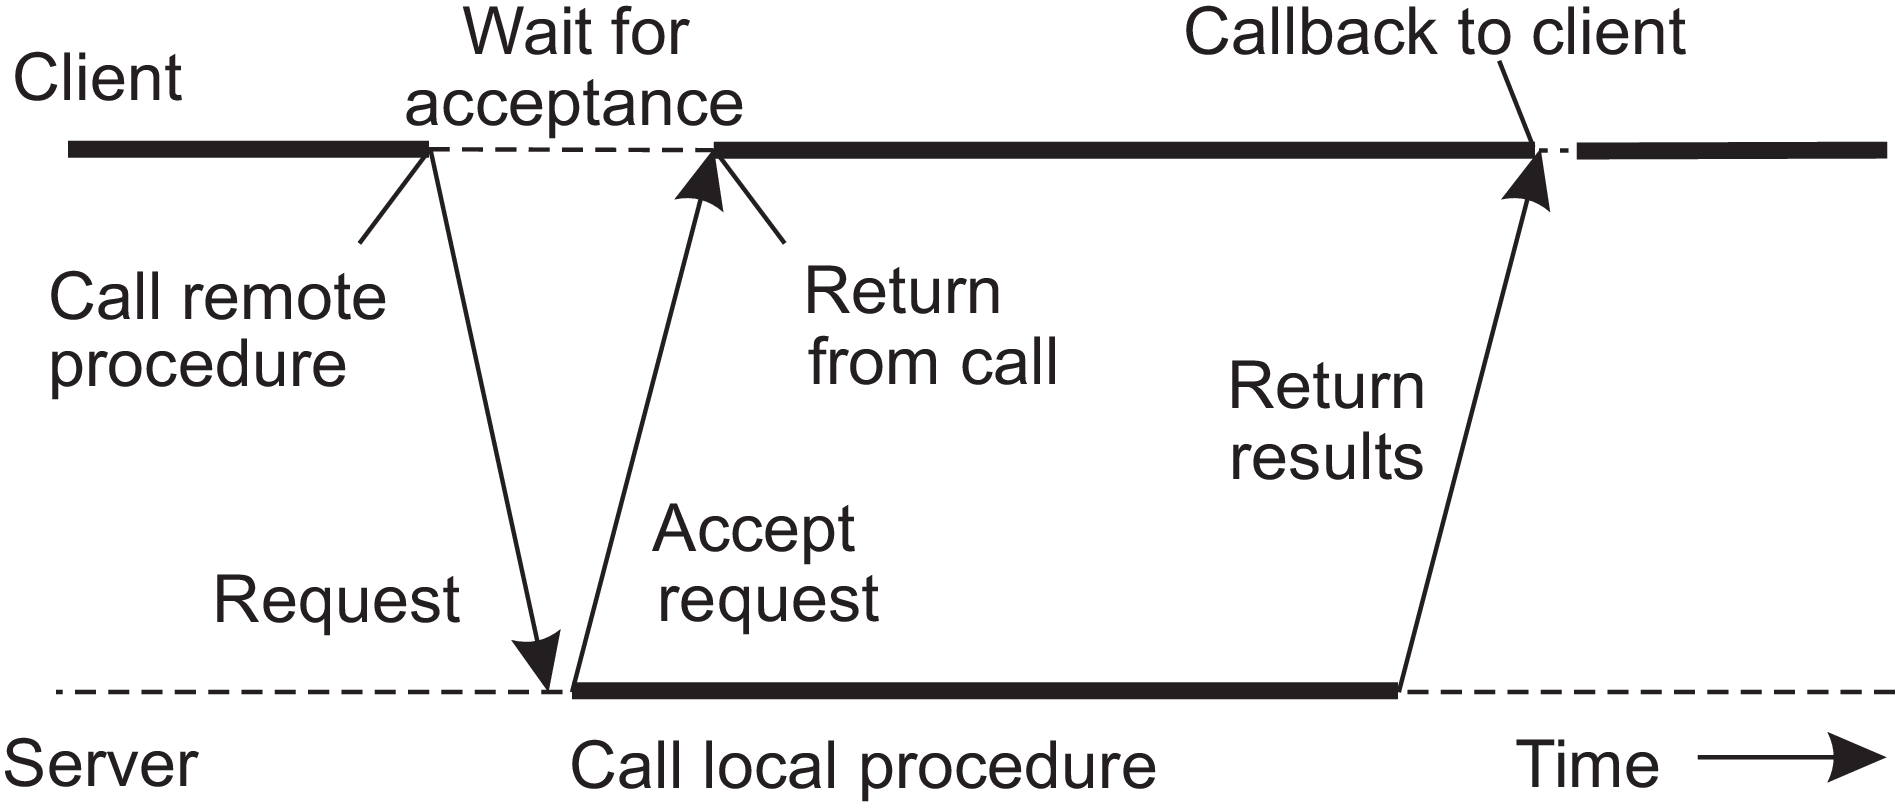
\includegraphics[width=\textwidth]{images/rpc_assincrona.png}

\end{frame}

%% --------------------------------------------------------

\begin{frame}{RPC multicast}

\vspace{0.5cm}

\centering 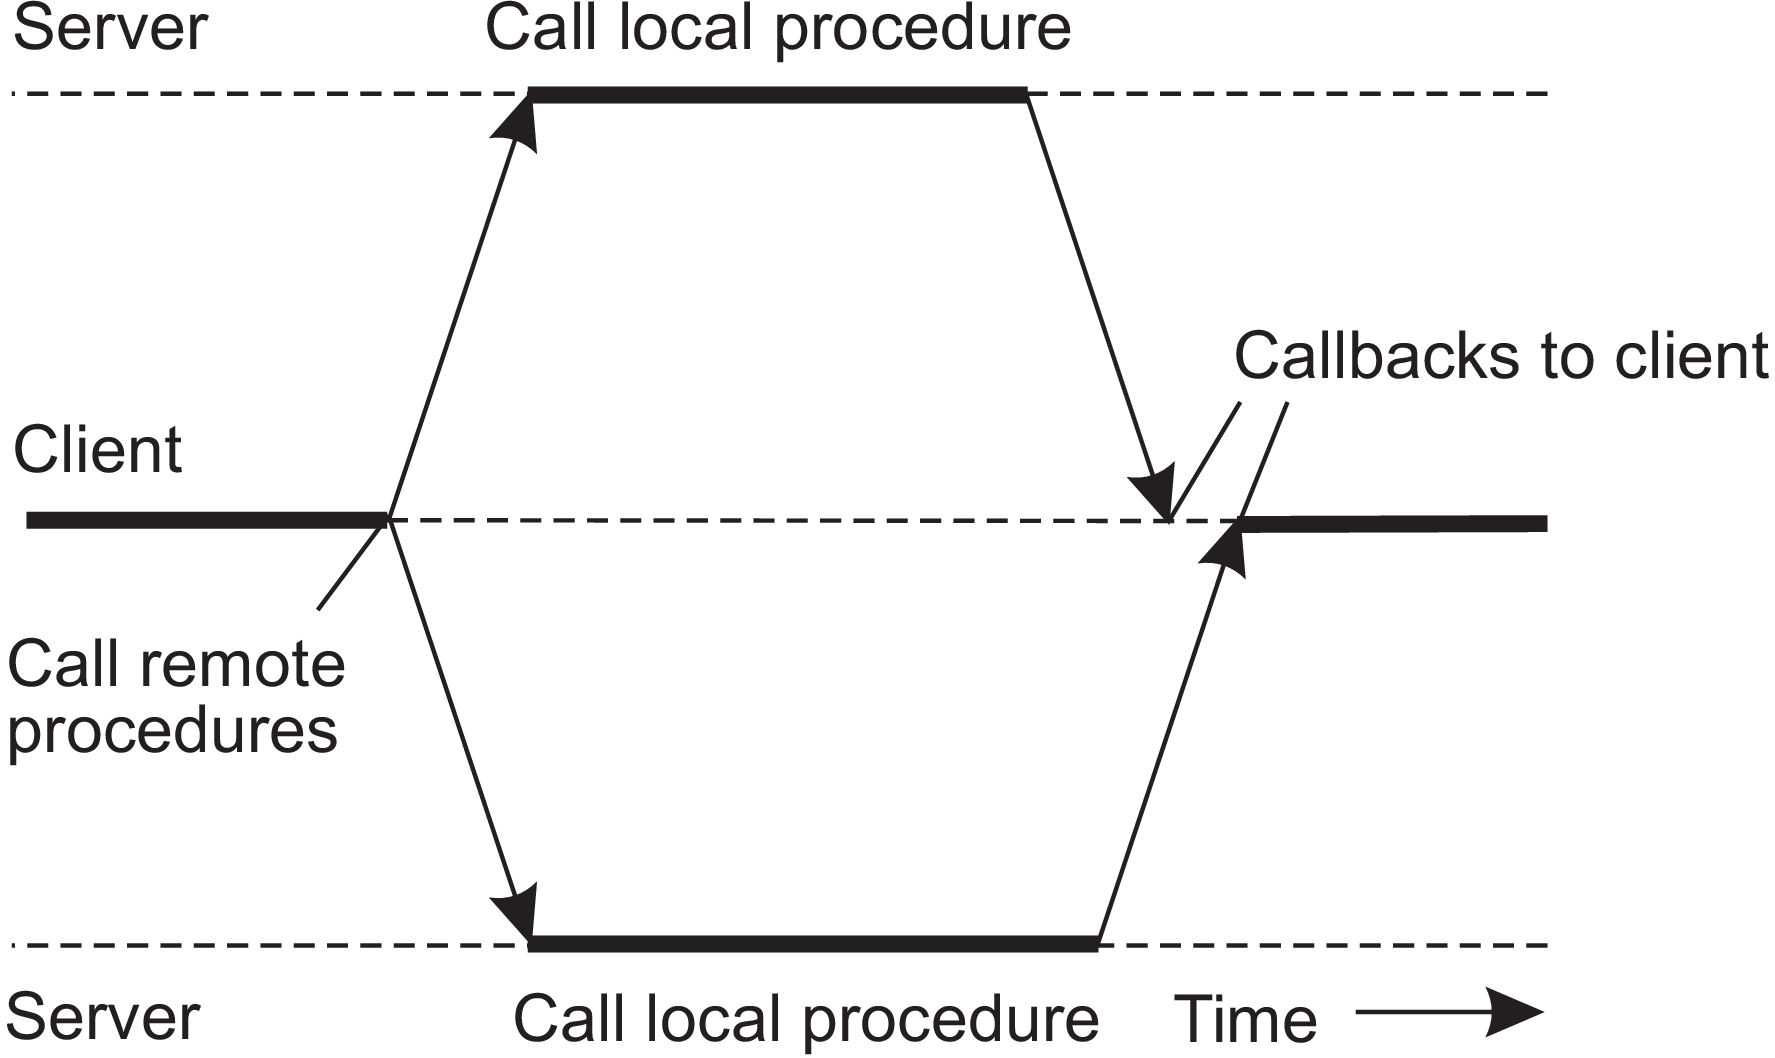
\includegraphics[width=\textwidth]{images/rpc_multicast.png}

\end{frame}

\end{document}
